\section{Experimental evaluation}\label{sec:experiments}

The experiments proposed in the previous sections were run on the OGBN-ArXiv dataset (see \cite{hu_open_2021}) with node2vec as the underlying graph learning algorithm. The experiments build upon the SOTA node2vec implementation for this dataset.

\subsection{Experiment setup}

The configurations of both the node2vec and the MLP models are taken from the PyTorch Geometric implementation of node2vec on the ogbn-arxiv dataset (a dataset of 169 343 computer science arXiv papers, see \cite{paszke_pytorch_2019}), which was also used for the experiments. The node2vec model generated an embedding into \( \mathfield{R}^{128} \) from \( 10 \) random walks of length \( 80 \) for each node with a context window size of \( 20 \). The optimizer ADAM \cite{kingma_adam:_2017} was used with a learning rate of \( 0.01 \) and batches of \( 256 \) samples. The MLP classifier using the embeddings featured \( 3 \) linear layers of \( 256 \) neurons with batch normalization after each layer. Finally, a linear layer was used for the class prediction. ADAM with a learning rate of \( 0.01 \) and a dropout rate of \( 0.5 \) was used for \( 200 \) epochs of training with the cross-entropy loss function. The experiments were implemented using PyTorch\footnote{https://pytorch.org/} and PyTorch Geometric \cite{paszke_pytorch_2019}.

\subsection{Effect of HARP pretraining}

\begin{table}
  \centering
  \begin{tabular}{lrr}
    \toprule
    Graph     & \# of nodes & \# of edges \\
    \midrule
    \( G_0 \) & 169 343     & 2 315 598   \\
    \( G_1 \) & 67 496      & 1 886 875   \\
    \( G_2 \) & 29 408      & 1 558 368   \\
    \( G_3 \) & 15 039      & 1 252 276   \\
    \( G_4 \) & 9 273       & 815 493     \\
    \( G_5 \) & 6 768       & 433 795     \\
    \( G_6 \) & 5 607       & 197 876     \\
    \( G_7 \) & 4 994       & 86 307      \\
    \( G_8 \) & 4 655       & 42 441      \\
    \( G_9 \) & 4 404       & 29 167      \\
  \end{tabular}
  \caption{Size of the graphs generated at different coarsening levels.}\label{tab:graph-sizes}
\end{table}

\begin{figure}
  \centering
  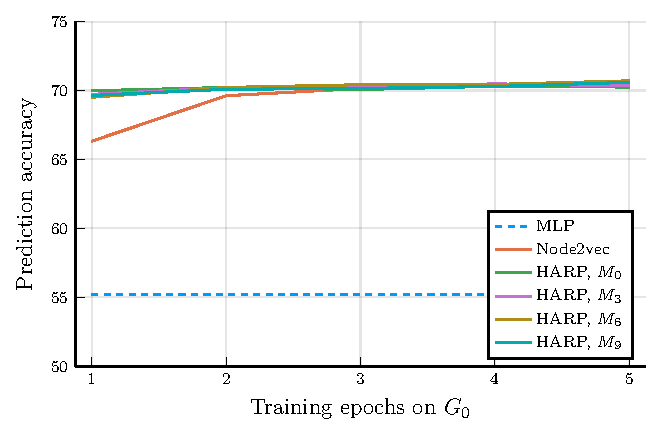
\includegraphics[width=0.8\textwidth]{images/steps_accur/steps_accur.pdf}
  \caption{Performance over epochs of models pretrained on different coarsening levels.}\label{fig:steps-accuracy}
\end{figure}

To asses the effect of HARP as a pretraining, the main question is how does HARP pretraining change the behaviour of the node2vec training? To this end, 10 different models \( M_0, \dots, M_9 \) as defined in Section \ref{sec:performance-vs-complexity} were trained. The sizes of the respective graphs \( G_0, \dots, G_9 \) are denoted in Table \ref{tab:graph-sizes}.

Figure \ref{fig:steps-accuracy} compares the accuracy of several models over learning epochs on the original graph \( G_0 \). An MLP using just dataset features and an ordinary node2vec model are provided as a reference. The models \( M_0, \dots, M_9 \) are then compared.

As can be seen, there is no noticeable difference in the performance of a pretrained node2vec in comparison to an ordinary one when it comes to performance after 4 or more training epochs. Our explanation is that the configuration used for node2vec training already samples large parts of the graph thanks to a relatively high number of long random walks. There is, however, a noticeable improvement in the performance of models when only very few training epochs are available.

\subsection{Feasibility of partially injective transformations}\label{sec:harp-vs-pihom}

\begin{figure}
  \centering
  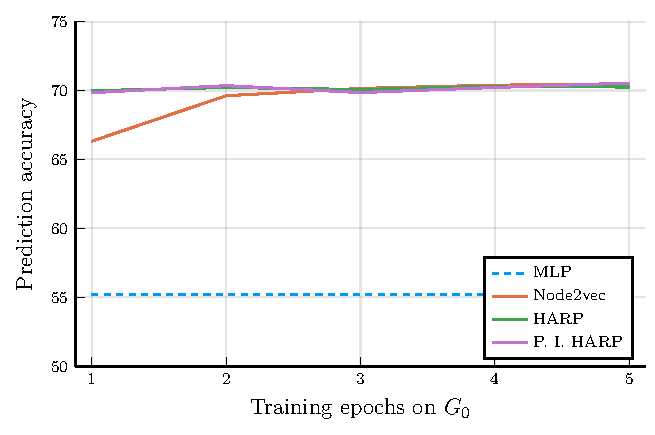
\includegraphics[width=0.8\textwidth]{images/pihom_comparison/pihom_comparison.pdf}
  \caption{Standard HARP compared to the version built on partially injective homomorphisms.}\label{fig:HARP-vs-PIHom}
\end{figure}

In order to test the feasibility of HARP-like algorithms based purely on partially injective homomorphisms, ordinary HARP is compared to one with the coarsening proposed in Section \ref{sec:harp-as-pihom}. Figure \ref{fig:HARP-vs-PIHom} shows the performance of such a model compared to ordinary HARP, node2vec and purely feature-based MLP classifier. As can be seen, there is no meaningful difference between the two models.
